% !TEX root = ../../buch.tex
% problemstellung.tex -- Beispiel-File für die Beschreibung des Problems
%
% (c) 2020 Prof Dr Andreas Müller, Hochschule Rapperswil
%
\section{Resultate
\label{burgers:section:results}}
\rhead{Resultate}

	Folgend werden die Berechnungen f\"ur eine Normalverteilte Startbedingung mit der expliziten und impliziten Methode gezeigt.
	Um den Vergleich zwischen den verschiedenen Methoden besser aufzuzeigen, werden die Resultate in 2-D aufgezeigt.
	F\"ur jeden Zeitschritt wird einen neuen Subplot gezeigt.
	
	\subsection{Explizit}

	Beim Expliziten Verfahren werden die beiden linearen Varianten aufgezeigt.
	Wobei sich nur der gew\"ahlte Punkt f\"ur die Multiplikation unterscheidet.
	In \ref{burgers:fig:ex} zeigen sich die Unterschiede welche durch eine marginal wirkende \"Anderung hervorgerufen werden.
	

    \begin{figure}
	\centering
	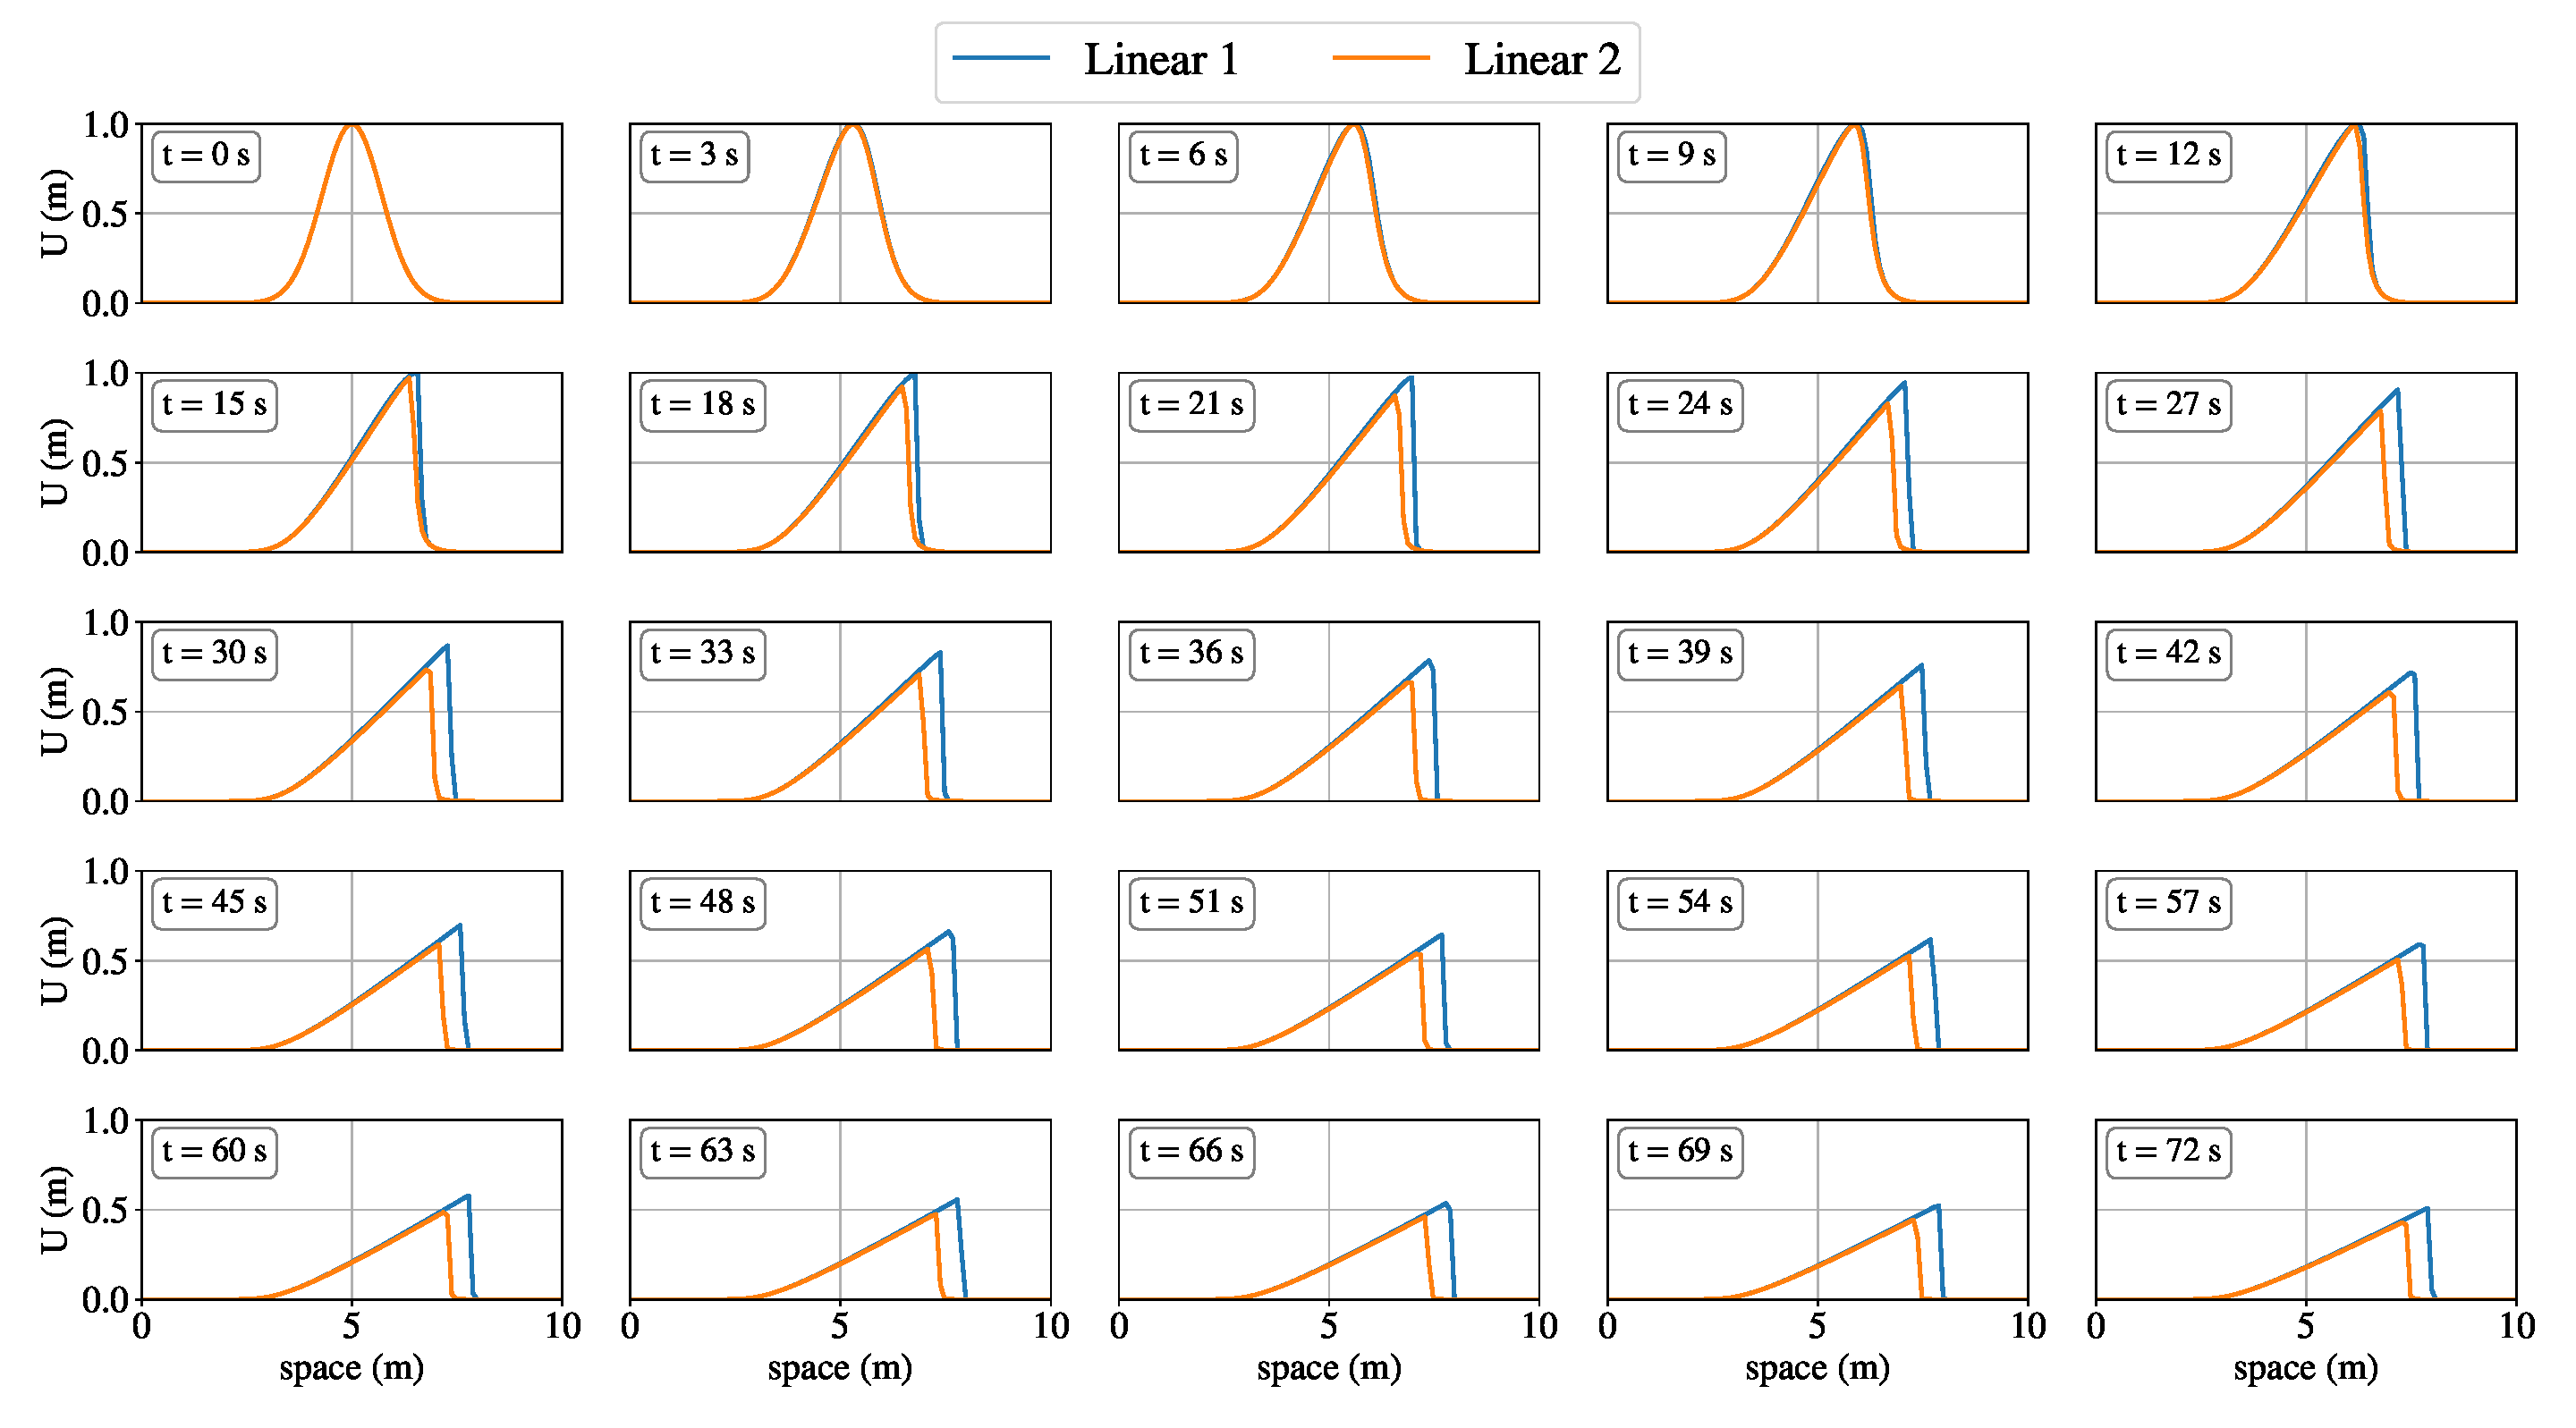
\includegraphics[width=1\textwidth]{papers/burgers/BurgersEquation/lin_paper.pdf}
	\caption{L\"osung Explizit}
	\label{burgers:fig:ex}
	\end{figure}
	
	\subsection{Implizit}

	Die Unterschiede bei den impliziten Verfahren sind in \ref{burgers:fig:imp} etwas besser ersichtlich.
	Es zeigt, dass der gew\"hlte Punnkt f\"ur die Ableitung bei der Leap-Frog Methode einen gr\"osseren Einfluss hat.
	Die Welle verh\"ahlt ist etwas tr\"ager als die beiden anderen Varianten.

    \begin{figure}
	\centering
	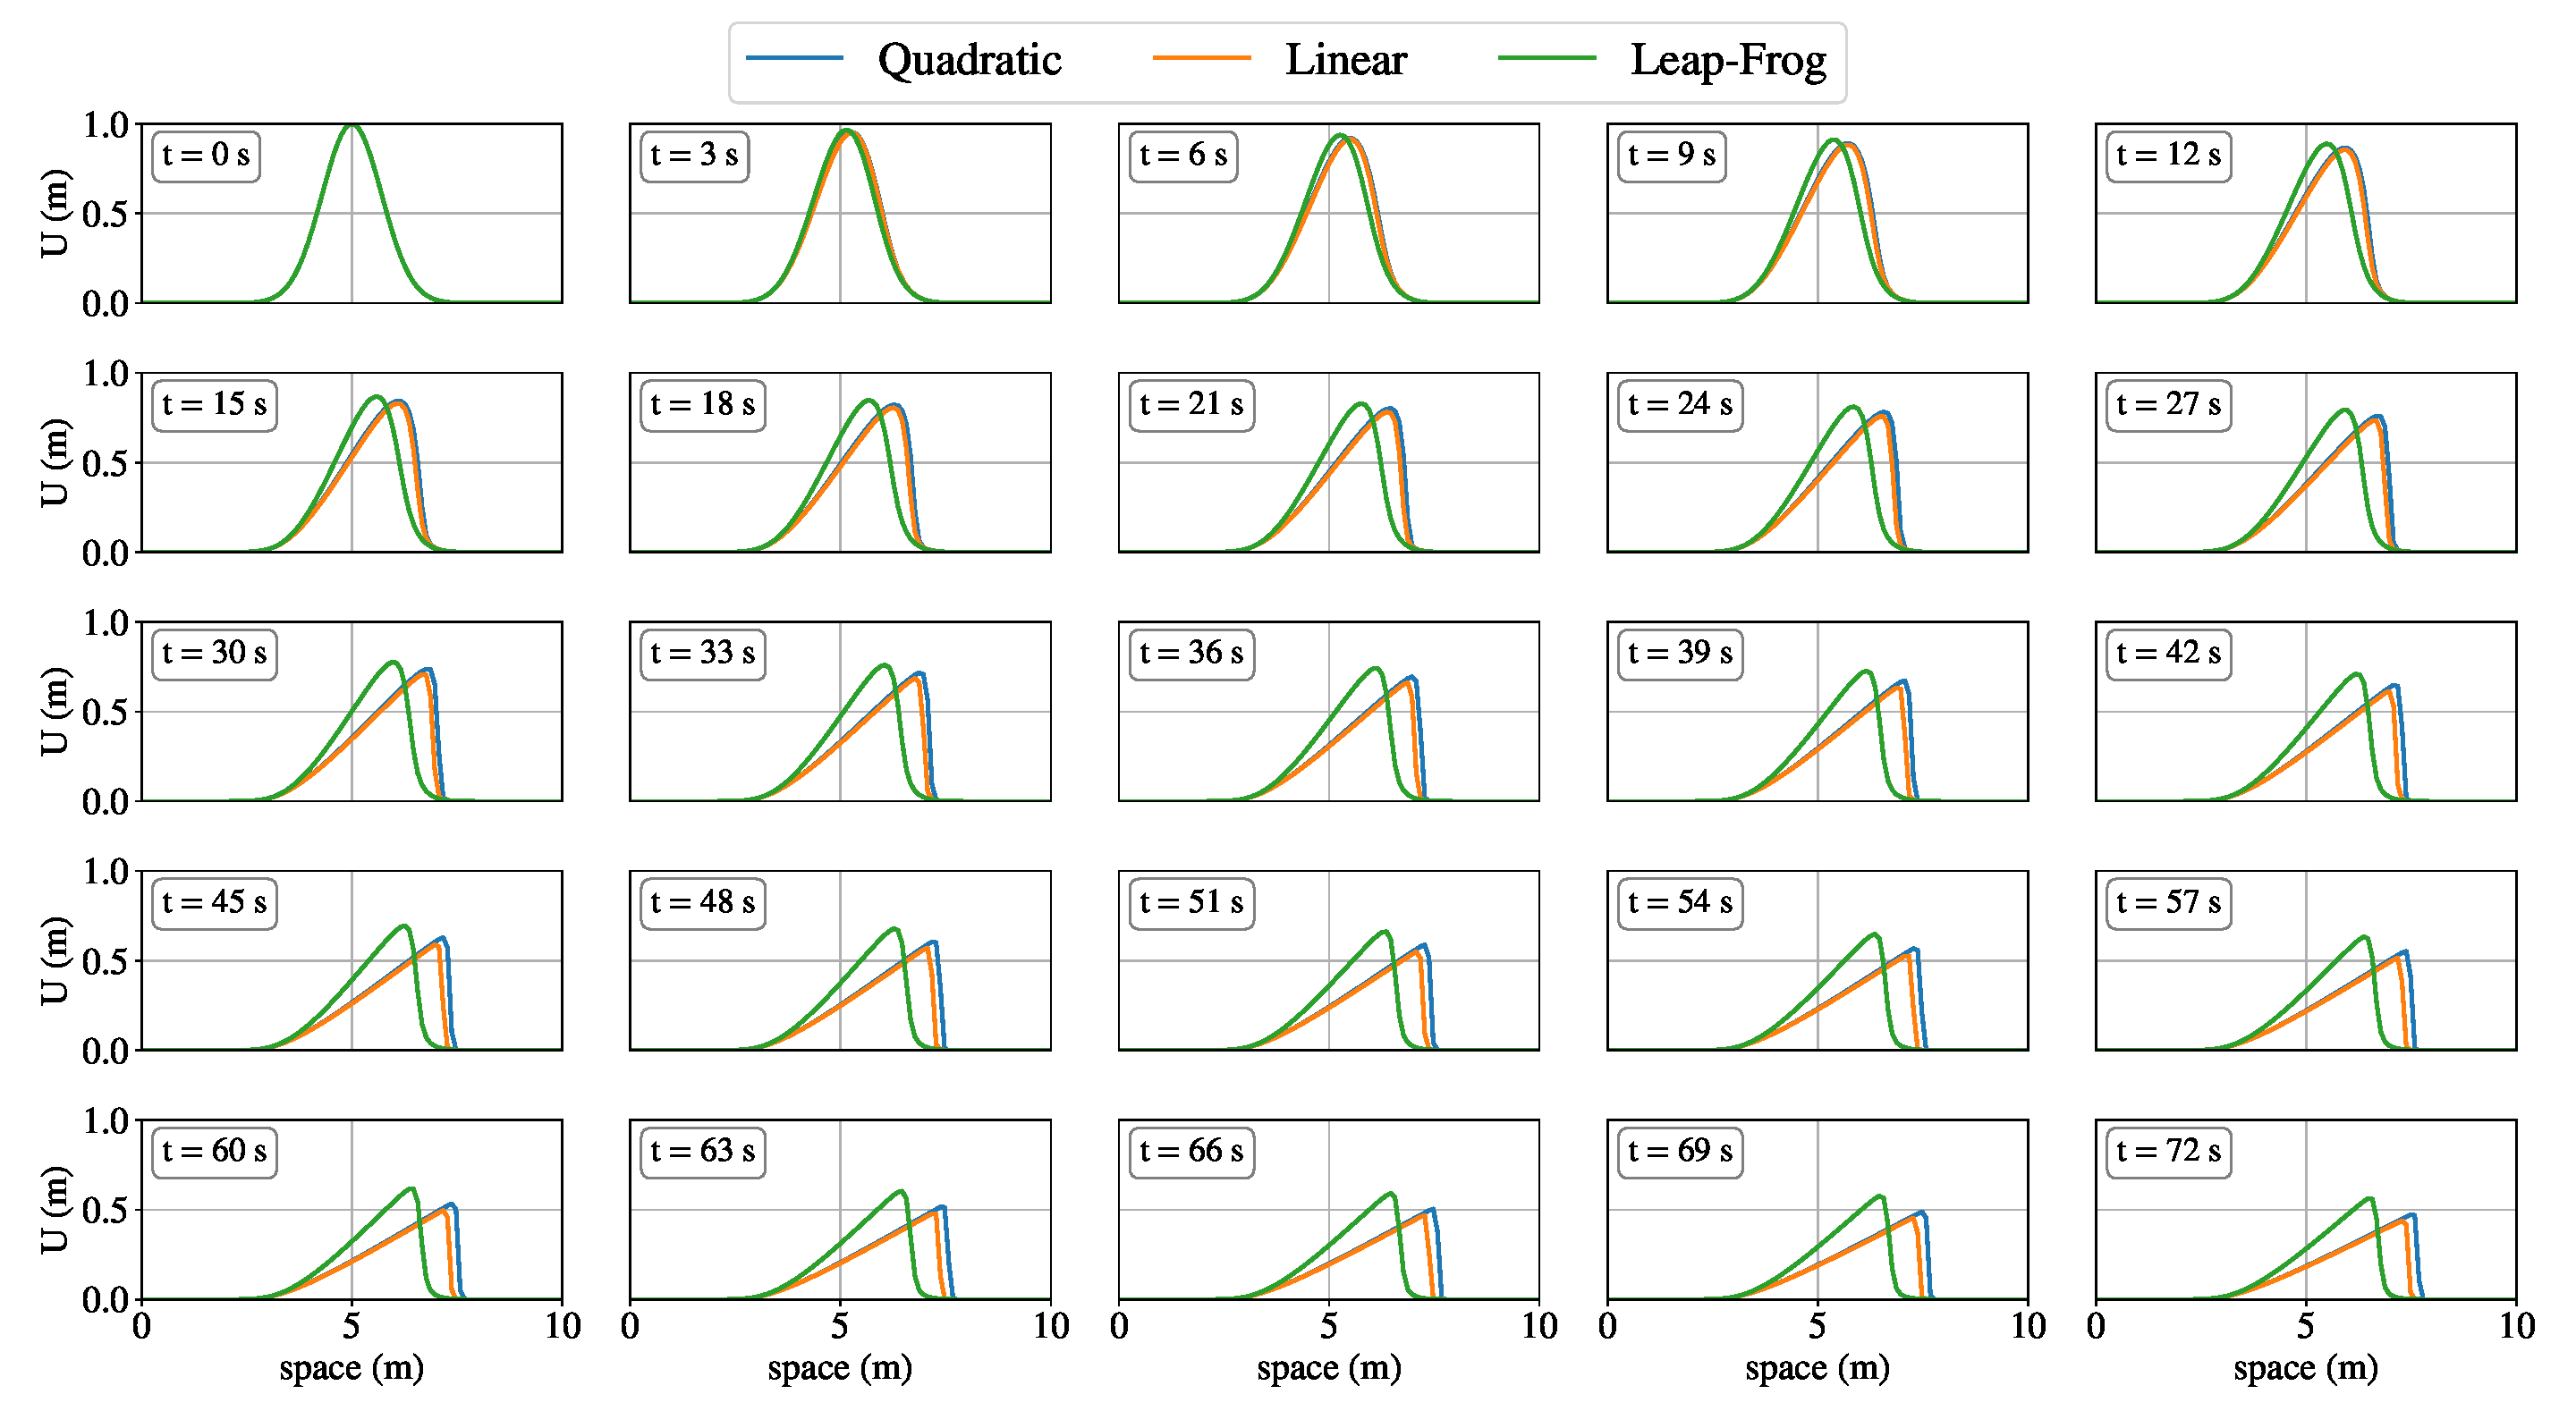
\includegraphics[width=1\textwidth]{papers/burgers/BurgersEquation/imp_paper.pdf}
	\caption{L\"osung Implizit}
	\label{burgers:fig:imp}
	\end{figure}
